% -*- TeX-engine: xetex; TeX-PDF-mode: t -*-

\documentclass{matmex-diploma-custom}
\begin{document}

\filltitle{ru}{
    chair              = {Кафедра Системного Программирования},
    title              = {Анализ эмоциональной окраски сообщений в микроблогах с помощью вероятностных моделей},
    type               = {diploma},
    position           = {студенки},
    group              = 545,
    author             = {Лебедева Екатерина Андреевна},
    supervisorPosition = { },
    supervisor         = {Тузова Е.\,А.},
    reviewerPosition   = { },
    reviewer           = { },
    chairHeadPosition  = {д.\,ф.-м.\,н., профессор},
    chairHead          = {Терехов А.\,Н.},
%   university         = {Санкт-Петербургский Государственный Университет},
%   faculty            = {Математико-механический факультет},
%   city               = {Санкт-Петербург},
   year               = {2014}
}

\filltitle{en}{
    chair              = {Chair of Software Engineering},
    title = {A probabilistic models for sentiment analysis of microblogging data},
    author             = {Ekaterina Lebedeva},
    supervisorPosition = { },
    reviewerPosition   = { },
    reviewer           = { },
    chairHeadPosition  = {professor},
    chairHead          = {Andrey Terekhov},
}
\maketitle
\tableofcontents

% Введение
%% -*- ispell-language: russian -*-

\section*{Введение}

Не так давно грань между потребителями и создателями информации в интернете
исчезла: на смену статическим страницам у всех пользователей появилась
возможность публиковать свою информацию. Сейчас мы наблюдаем огромное
количество видов создаваемых материалов. Это может быть запись
в блоге или на форуме, фотография или видеозапись на соответствующем
ресурсе, отзыв в интернет-магазине,``статус'' в социальной сети и многое другое.
Совершенная простота размещения текстов от разных людей в одном месте
в интернете стала поводом для появления всевозможных вебсайтов, собирающих мнения
пользователей, например, о книгах, фильмах, товарах, и вот некоторые из них:
epinions.com, rottentomatoes.com, amazon.es, market.ya.ru. Прежде, чем что-то приоберсти,
покупатель ищет отзывы о серии необходимых товаров в интернете, он читает
десятки мнений различных людей, а на основании этих мнений делает вывод о том,
какой же продукт ему действительно подходит, и только после этого что-то покупает.
Со временем текстов стало так много, что обработать все их за разумное время человеку просто
не по силам. Именно такая ситуация стала причиной возникновения
задачи анализа мнений: появилась необходимость в создании системы для
автоматического поиска, классификации и представления точек зрения.

Анализ мнений -- одно из направлений области обработки текстов на естественных
языках. Саму задачу можно определить как вычислительное выявление
субъективности в текстах и отношения авторов этих текстов к некоторым объектам.
Изначально в качестве исследуемых данных использовались большие записи,
состоящие из нескольких предложений, в которых явно прослеживались связь и
контекст. Позже, с развитием социальных сетей, с появлением в них комментариев,
``статусов'' и  коротких сообщений, пользовательский контент стал менее ёмким,
но при этом более субъективным и превратился в бесконечный поток поступающей
информации. Ярким примером этому является сервис микроблогов
Twitter (http://twitter.com) (Твиттер). С помощью этого сервиса пользователи распространяют
свои взгляды на актуальные новости, связанные с разными интересными
другим людям областями, такими как политика, экономика, бизнес и другие,
рассказывают о купленных товарах, а также публикуют личную информацию, например,
что они сейчас делают и в каком настроении находятся.

В этой работе речь пойдёт именно о сообщениях, характерных для Твиттера.
Отличительная особенность этой платформы в том, что у пользователя есть
только 140 символов, чтобы выразить свои мысли или отношение к чему-либо.
Каждое сообщение, называемое здесь ``твит'' и публикуемое пользователем в
Твиттере, могут увидеть его подписчики -- люди, которые связаны с ним в этой
социальной сети. Подписчики (или иначе ``читатели'') могут быть как
односторонними, так и взаимными. Если человек увидел зинтересовавший его твит
и разместил его на своей странице, то говорят, что он ретвитнул
запись другого пользователя. В этом случае информация распространяется не только
на подписчиков первоначального автора, но и на читателей того, кто сделал
ретвит. Есть и другой вид взаимодействия пользовательской
информации: упоминания. Если читатель захотел ответить на какой-либо твит,
он это делает, вставив в начало своего сообщения псевдоним автора в Твиттере при помощи
символа @ (@username), тем самым, упоминая его. В этом случае ответ увидят
только те, кто читает обоих дискутирующих пользователей. Если упоминание
происходит в середине твита, то он доступен точно так же, как и обычный,
только упомянутому пользователю приходит отдельное оповещение.
Механизмов социального взаимодействия в Твиттере больше нет, но этого достаточно,
чтобы информация распространялась очень быстро и охватывала большую аудиторию.

Основной способ представления твитов -- это представление в виде ленты.
Пользователь, войдя на сайт, видит сообщения от всех читаемых им людей,
отсортированные в порядке удаления времени от настоящего момента. Дальше
он может перейти на страницу конкретного человека и прочитать только его
сообщения,  но обычно информация воспринимается именно в форме потока,
уходящего назад, до момента регистрации читающего пользователя на сайте.
Так он узнаёт, что нового произошло в жизни его знакомых, о чём рассказывают
интересные ему аккаунты и какие события обсуждаются в мире. При помощи ретвитов
информация действительно распространяется очень быстро. Например, можно
вспомнить ситуацию с (лучше какая-нибудь научная утка)

Кроме чтения релевантных сообщений от читаемых пользователей, можно
пользоваться поиском по хештегу. Хештег -- специальное слово, перед которым
стоит символ \# (\#хештег). Наличие хештега подразумевает, что твит имеет какое-то
отношение к объекту, обозначаему этим словом. Поиск по хештегам учитывает
записи всех пользователей, поэтому количество получаемой информации здесь не
просто большое, оно настолько велико, что страница с выдачей по популярным
запросам почти никогда не является актуальной. Твиты в выдаче также организованы
по принципу временной ленты, отдаляющейся от настоящего момента, поэтому, как
только пользователь пишет новый запрос, кто-то публикует запись с этим же хештегом.
Проблема даже не в том, что появляются новые твиты, а в том, что пользователь не
успевает обработать все существующие. Хештег -- это способ явно указать объект, о
котором идёт речь в сообщении, но не все пользователи их ставят, поэтому поиск
по ключевым словам даёт более полную информацию, хотя иногда и не носящую смысла,
а её количество уж тем более становится неподъёмным.

Что же можно делать с огромным количеством коротких текстов на определённую
тему, носящих, в основном, субъективный характер и не помещающихся вместе
в голове обычного человека? Точнее, что можно хотеть с ними делать? Вот пример:
выходит обновление какого-нибудь известного ПО, и компания публикует об этом
новость на своей странице в Твиттере. Читатели Твиттера этой компании воспринимают
сообщение о новой версии продукта и, во-первых, сами о ней узнают, во-вторых,
могут ретвитнуть её для своих подписчиков, и к аудитории новости присоединятся другие пользователи,
в-третьих, могут прокомментировать и показать тем самым своё отношение к событию.
На всех этапах распространения информации о продукте компании важно, какую
эмоциональную окраску она носит. В такой ситуации понятно, в какой момент и что
надо отслеживать. Но бывает, что человек написал в своём Твиттере мнение о
продукте независимо от публикаций компании или её представителей. Тут уже
начинается исследование эмоциональной окраски не среди комментариев к твитам и
ретвитам конкретной записи, а в целом среди текстов, имеющих отношение к целевому
объекту. Такая же задача встаёт, когда речь идёт об объектах из других областей:
всё те же политика, экономика, события в обществе и прочее.

Таким образом, ставится задача разметить в соответствии с эмоциональной окраской
множество твитов, имеющих отношение к конкретному объекту, заданному словом или
словосочетанием, с использованием особенностей именно этой социальной сети. Подобную
задачу решают и для больших текстов при помощи лигвистического словарного подхода и
вычислительно, методами машинного обучения. Цель данной работы --
исследовать проблему для Твиттера и предложить вариант её решения с использованием
аппарата вероятностных моделей.

Кроме Твиттера сервисами микроблогов отчасти явлюятся и другие социальные сети, например,
ВКонтакте (vk.com), Facebook (facebook.com), FourSquare (foursquare.com),
Instagram (instagram.com) поэтому задача, в целом, распространяема и на них,
но, так как эти платформы предоставляют много других возможностей, для ведения
микроблогов они используются гораздо меньше, чем Твиттер, и в этой работе
рассматриваться не будут.


% Обзор
\chapter{Обзор существующих решений}

\section{Конкретизация задачи}
Задача анализа эмоциональной окраски текстов сводится к задаче классификации. В
нашем случае имеется набор твитов, каждый из которых нужно отнести к одной из
трёх категорий: положительные, нейтральные или отрицательные.

Иногда классификация происходит в два этапа и на обоих этапах является бинарной.
На первом отделяются субъектиные сообщения от объективных. Объективными в этом
случае называются как раз те, которые не несут эмоциональной окраски и
явлются нейтральными варианте с тремя классами. Второй этап делит субъективные
тектсы на положительные и отрицательные. В случае с Твиттером, где почти все
сообщения субъективны, а критерии нейтральности можно сформулировать только в
смысле ``не положительное'' и ``не отрицательное'', будем использовать разделение
на три класса.

Твит -- это строка, состоящая из не более чем 140 символов. Он может содержать
специальные слова, начинающихся с определённых знаков: сразу после ``@'' пишется
имя пользователя, с которым сообщение связано или к которому оно обращено,
а после ``\#'' находится так называемый хештег -- слово, которое явно указывает
на связь твита с объектом, который этим словом обозначается. Все твиты создаются
пользователями, поэтому могут содержать опечатки, ошибки, сокращения,
особую пунктуацию и прочие способы выражения мысли в коротком тексте.
У каждого сообщения в Твиттере есть время, когда оно опубликовано, и автор.
Если один твит является ответом на другой, то у первого есть ещё и ссылка на второй,
то есть на ``родительский''. Ретвиты содержат также данные о первоначальном
размещении.

\section{Общий подход}
Вычислительно поставленная задача решается при помощи машинного обучения. Первое
упоминание анализа мнений в таком контексте относится к 2002 году. Тогда были рассмотрены
стандартные решения методом обучения с учителем \cite{pang2002thumbs} и
задачу для отзывов людей на специализированных ресурсах.
В первом случае за основу берутся лингвистические данные: словарь положительных
и словарь отрицательных слов. Во втором -- набор отзывов, уже разделённых на
положительные и отрицательные.

% Решение
\section{Особенности задачи для данных из микроблогов}
\subsection{Основные характеристики данных}
Микроблоги --- это, в первую очередь, сервисы для упрощения публикации и восприятия пользовательских
данных. Обычно сообщения в микроблогах состоят из одного или пары предложений, а для Твиттера есть
строгое ограничение на длину твита --- 140 символов. В 140 символов пользователям платформы необходимо
уместить контекст, своё отношение к теме и, возможно, ссылку на фотографию, Интернет-ресурс или
другой медиа объект. Часто контекст восстанавливается из окружающего мира, то есть пользователь
пишет о том, что волнует Интернет в этот момент, и люди, владея этой информацией, сопоставляют
высказывание с реальными событиями. У компьютера так просто быть в курсе обсуждаемых тем не
получается, поэтому на восстановление контекста рассчитывать не приходится.

Платформы для ведения микроблогов также являются социальными сетями, где пользователи могут
взаимодействовать друг с другом. В Твиттере, например, кроме социальных графов можно наблюдать
графы, в которые выстраиваются сами сообщения: пользователи могут отвечать на твиты, а также
размещать у себя твиты других пользователей, в терминологии платформы это называется
<<ретвитить>>. Информация о социальных взаимодействиях может уточнять результаты классификации,
например, есть интуитивное предположение, что ответ на отрицательно окрашенное сообщение тоже
попадёт в класс негативных.

\subsection{Особенности текстов}
\subsubsection{Смайлы}
Для выражения эмоций в тексте пользователи ставят смайлы. Смайл --- это набор символов, условно
иллюстрирующий выражение лица автора, а точнее его настроение. Все смайлы можно поделить на
восточные и западные по географии их использования, последние приведены в таблице \ref{tab:smileys}
с метками, соответствующими их эмоциональной окраске. В случае с короткими текстами нет более
простого способа отметить своё отношение к теме, чем поставить смайл, но не все пользователи так
делают, поэтому размечать сообщения с их помощью в общем случае не получится. Есть и более сложные
конструкции из скобок, двоеточий и других симовлов, но они используются не так часто и обычно
означают уже не просто отношение, а какие-то действия или объекты, то есть эмоциональной окраски не
несут.

\begin{table}[h]
\begin{tabular}{|cc|cc|cc|cc|cc|}
\hline
\textbf{Смайл}              & \textbf{Метка} & \textbf{Смайл}         & \textbf{Метка} & \textbf{Смайл}   & \textbf{Метка} & \textbf{Смайл} & \textbf{Метка} & \textbf{Смайл} & \textbf{Метка} \\ \hline
:-)                         & +              & :)                     & +              & :o)              & +              & :{]}           & +              & :3             & +              \\
:c)                         & +              & :\textgreater          & +              & ={]}             & +              & 8)             & +              & =)             & +              \\
:\}                         & +              & :\textasciicircum )    & +              & :>)              & +              & :-D            & +              & :D             & +              \\
8-D                         & +              & 8D                     & +              & x-D              & +              & xD             & +              & X-D            & +              \\
XD                          & +              & =-D                    & +              & =D               & +              & =-3            & +              & =3             & +              \\
B\textasciicircum D         & +              & :-))                   & +              & \textgreater:{[} & -              & :-(            & -              & :(             & -              \\
:-c                         & -              & :c                     & -              & :-\textless      & -              & :>C            & -              & :\textless     & -              \\
:-{[}                       & -              & :{[}                   & -              & :\{              & -              & ;(             & -              & :-||           & -              \\
:@                          & -              & \textgreater:(         & -              & :’-(             & -              & :’(            & -              & :’-)           & +              \\
:')                         & +              & D:\textless            & -              & D:               & -              & D8             & -              & D;             & -              \\
D=                          & -              & DX                     & -              & v.v              & -              & D-‘:           & -              & :*             & +              \\
:\textasciicircum *         & +              & (                      & +              & \}\{            & +              & )              & +              & ;-)            & +              \\
;)                          & +              & *-)                    & +              & *)               & +              & ;-{]}          & +              & ;{]}           & +              \\
;D                          & +              & ;\textasciicircum )    & +              & :-,              & +              & \textgreater:P & +              & :-P            & +              \\
:P                          & +              & X-P                    & +              & x-p              & +              & xp             & +              & XP             & +              \\
:-p                         & +              & :p                     & +              & =p               & +              & :-Þ            & +              & :Þ             & +              \\
:þ                          & +              & :-þ                    & +              & :-b              & +              & :b             & +              & d:             & +              \\
\textgreater:\textbackslash & -              & \textgreater:/         & -              & :-/              & -              & :-.            & -              & :/             & -              \\
:\textbackslash             & -              & =/                     & -              & =\textbackslash  & -              & :L             & -              & =L             & -              \\
:S                          & -              & \textgreater.\textless & -              & :|               & -              & :-|            & -              & :\$            & -              \\
O:-)                        & +              & 0:-3                   & +              & 0:3              & +              & 0:-)           & +              & 0:)            & +              \\
0;\textasciicircum )        & +              & O\_O                   & -              & \o/              & +              & \textless3     & +              & \textless/3    & -              \\ \hline
\end{tabular}\caption{Эмоциональная окраска смайлов.}\label{tab:smileys}
\end{table}

\begin{figure}[h]
\centering
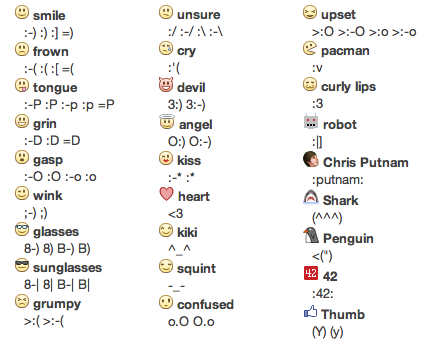
\includegraphics[width=0.5\textwidth]{ListofFacebookChatEmoji}
\caption{Некоторые графические смайлы, используемые в Facebook.}
\label{emoji}
\end{figure}

\pagebreak
Кроме ASCII смайлов есть ещё и графические --- это картинки, которые вставляются в текст. В
современных веб-сервисах и мобильных приложениях используется графический язык Emoji\footnote{www.emoji-cheat-sheet.com} для
записи слов, эмоций и действий. На рисунке \ref{emoji} изображены некоторые известные графические
смайлы, которые используются в социальной сети Facebook\footnote{facebook.com}. Обычно для
каждого из них есть ASCII аналог, причём не один. Набирая сообщение на клавиатуре компьютера или
ноутбука, удобнее поставить двоеточие со скобкой, но смартфоны и планшеты предоставляют все удобства
для вставки улыбчивых картинок: наряду с русской и английской клавиатурой, например, на них можно
подключить и клавиатуру графического языка Emoji.

Так как смайлы являются своего рода разметкой сообщений самими пользователями, их необходимо
использовать при анализе эмоциональной окраски. В этой работе будет рассмотрено применение
символьных и графических улыбок для сбора корпуса твитов и для предобработки данных непосредственно
перед классификацией.

\subsubsection{Хештеги}

Ещё одна особенность общения в микроблогах --- хештеги. Пользователь помечает в своём сообщении
слово, ставя перед ним <<\#>>, тем самым показывая связь объекта, обозначаемого этим словом, и всего
твита. Платформы для микроблогов предлагают возможность искать по хештегам, выбирать из них
популярные и следить за потоками актуальной информации. Многие хештеги используются в течение
короткого периода времени, но затем именно по ним можно найти информацию, которая когда-то была
актуальной и понадобилась через несколько месяцев. Например, организаторы мероприятий стараются
придумывать уникальный хештег, размещать его на информационных стендах, чтобы участники следили за
твитами друг друга и распространяли информацию по всему Интернету. Можно сказать, что это
повествовательная функция хештегов, точнее, тех из них, которые указывают на объект,~--- они могут
помочь осуществлять поиск сообщений на определённую тему.

Другую функцию этих специальных слов-ассоциаций можно назвать описательной. Именно такие хештеги
можно использовать в определении эмоциональной окраски текстов. В работе
\cite{qadir2013bootstrapped} предложен способ классифицикации хештегов по их эмоциональной
окраске. Авторы предлагают читателям посмотреть на 20 самых популярных хештегов из каждой
группы. Для наглядности в таблице \ref{tab:hashtags} приведены первые пять для каждой эмоции.

\begin{table}[h]
  \begin{tabular}{|c|c|c|c|c|} \hline
    \textbf{Привязанность} & \textbf{Ярость} & \textbf{Страх} & \textbf{Наслаждение} & \textbf{Грусть}\\ \hline
    \#youthebest&\#godie&\#hatespiders&\#thankinggod&\#catlady\\
    \#yourthebest&\#donttalktome&\#freakedout&\#thankyoulord&\#buttrue\\
    \#hyc&\#fuckyourself&\#creepedout&\#thankful&\#singleprobs\\
    \#yourethebest&\#getoutofmylife&\#sinister&\#superexcited&\#singleproblems\\
    \#alwaysandforever&\#irritated&\#wimp&\#tripleblessed&\#lonelytweet\\
    \hline
  \end{tabular}
  \caption{Самые популярные хештеги для пяти чувств: привязанности, ярости, страха, наслаждения и
    грусти. }\label{tab:hashtags}
\end{table}

Использование хештегов непосредственно для оценки эмоциональной окраски можно считать примерно таким
же, как и у смайлов, но лишь тогда, когда слово однозначно относится либо к положительным,
либо к отрицательным. В противном случае они либо становятся обычными словами: без символа <<\#>>
они участвуют в классификации наравне с другими, либо уточняют вероятность сообщения попасть в тот
или иной класс при помощи подсчёта условных вероятностей, где условием и является хештег.

\subsubsection{Сокращения, пролонгирования и пунктуация}
Тексты в микроблогах содержат не только уточняющую информацию, но и отчасти мешающую. Её нужно научиться использовать, так как
специфика сообщений не позволяет хоть что-то выкидывать.

Ограничение в 140 символов заставляет людей сокращать слова, причём как при помощи общеизвестных
аббревиатур, например, <<СПбГУ>> --- это Санкт-Петербургский Государственный Университет, так и при
помощи жаргонных конструкций: <<h8>> --- это на самом деле hate. На примере последнего видно, что
избавиться от этого слова было бы расточительно, но вряд ли <<h8>> внесло бы вклад в
вероятность сообщения попасть в класс отрцательных такой же, как и слово <<hate>>. Получается,
сокращения нужно уметь переводить.

Когда пользователям кажется, что длина сообщения не такая уж и маленькая, они используют
пролонгирования гласных --- ещё один способ выражать обеспокоенность темой твита. Автор преумножает
гласную в слове, изображая её продолжительное звучание, то есть, например, крик. Так <<nooooooo>>
будет, скорее всего, означать категорическое несогласие, а <<so cuuuute>> --- умиление. Таким
образом, каждое такое слово что-то значит, но классификатор может об этом не знать, значит, нужно
рассказывать классификатору какими-то другими способами, что это важное слово и какое из известных
является его менее эмоциональным аналогом.

Авторская пунктуация может рассказать об эмоциональной окраске сообщения не меньше, чем
смайлы. Например, в нейтральных твитах крайне редко встречаются восклицательные знаки. Впрочем,
однозначно классифицирующих особенностей пунктуации не так и много: наличие восклицательных знаков
указывает на наличие эмоциональной окраски, при этом нельзя без дополнительного анализа сказать,
какой именно; сочетание <<?!>>, скорее всего, будет означать недоумение, то есть классифицируется
как отрицательное; многоточия обычно говорят о нейтральности.

\subsection{Использование особенностей текстов для предобработки}\label{spec}
Смайлы, хештеги, сокращения, пролонгирования и пунктуация --- это то, про что классификатор уже не
знает, то есть перед подачей ему сообщения необходимо преобразовать это сообщение так, чтобы все
перечисленные особенности не выбивались и превратились в обычные слова.

Смайлы, перечисленные в таблице \ref{tab:smileys}, заменяются в тексте на соответствующую им
метку. Это делается для того, чтобы в обучающей выборке слово <<+>> встретилось больше раз среди
положительных твитов, тем самым, в вероятность попасть в класс положительных <<+>> даст больший
вклад, чем  просто <<:)>>. Так же, заменой на <<+>> и <<$\minus$>>, обрабатывается пунктуация.

К смайлам, заменяемым на метки, добавляется замена некоторых однозначно классифицирующихся
хештегов. Происходит это по той же причине, что и со смайлами. Если замена хештега не произошла, то
считается, что он должен стать обычным словом, то есть <<\#>> из начала пропадает, и дальше работа
происходит уже без учёта того, что это хештег.

Если в сообщении встречается неизвестное слово, его стоит проверить на наличие в словаре сокращений. В данной
работе используется словарь <<No slang>>\footnote{http://www.noslang.com/}, к которому программа
обращается во время подготовки данных к подаче классификатору. Запрос к словарю происходит в
онлайн-режиме, и для обработки сокращений нужно подключение к Интернету.

Повторения гласных убирать совсем не нужно: достаточно сократить количество повторяющихся гласных
до двух, то есть <<nooooooo>> заменится на <<noo>>. В этом случае слово <<noo>> может встретиться в
обучающей выборке, в отличие от <<nooooooo>>, где именно семь, а не восемь или девять букв
<<о>>. Таким образом слово <<no>> уже не то же самое, что <<noo>>, но все, сколько угодно длинные
продолжения гласной <<о>> сведутся к одному и тому же эмоциональному <<noo>>, которое даст каждому
из таких слов с продолжениями одинаковый повод попасть в класс <<$\minus$>>.


% Библиография
\bibliographystyle{ugost2008ls}
\bibliography{main}

\end{document}